%% LyX 1.6.7 created this file.  For more info, see http://www.lyx.org/.
%% Do not edit unless you really know what you are doing.
\documentclass[english]{article}
\usepackage[T1]{fontenc}
\usepackage[latin9]{inputenc}
\usepackage{varioref}
\usepackage{amstext}
\usepackage{graphicx}

\makeatletter

%%%%%%%%%%%%%%%%%%%%%%%%%%%%%% LyX specific LaTeX commands.
\newcommand{\noun}[1]{\textsc{#1}}
%% Because html converters don't know tabularnewline
\providecommand{\tabularnewline}{\\}
%% A simple dot to overcome graphicx limitations
\newcommand{\lyxdot}{.}


\makeatother

\usepackage{babel}

\begin{document}

\title{A Feed-Forward Neural Net for Parity Checking}


\author{Dennis Ideler}


\date{December 4th, 2009}

\maketitle
Computer Science Department, Brock University

COSC 3P71: Introduction to Artificial Intelligence

di07ty@brocku.ca, 4134466

\tableofcontents{}


\section{Introduction}

Neural networks are not a new concept; research on them has been going
on for some time. For instance, the McCulloch and Pitts neural model
dates back to the early 1940s and the perceptron%
\footnote{A single layer feed-forward neural network invented by \noun{Frank
Rosenblatt}.%
} was built back in the late 1950s. Unfortunately, interest declined
from the late 1960s until the 1980s, due to proofs and demonstrations
of the perceptron's limitations and computational weakness. Fortunately
for the sake of science, interest was raised again%
\footnote{See section~\vref{sub:Error-Backpropagation}~to find out why.%
} and research in this field continues at a healthy pace. Nowadays
neural networks have many uses and are used in many fields, such as
physics, psychology, statistics, engineering, econometrics, and computer
science to name a few.

The rest of the introduction includes a basic intro to the learning
system used and the problem at hand. If you already have a decent
understanding of both, you can skip the introduction.


\subsection{Artificial Neural Networks}


\subsubsection{What Are Artificial Neural Networks?}

Artificial neural networks (ANN), or simply neural networks (NN),
are adaptive statistical models based on an analogy with the structure
of the brain%
\footnote{Biological Neural Nets (BNN) are the natural {}``equivalent'' of
the ANN.%
}. Artificial neural networks are basically built from simple units
called \emph{(artificial) neurons}%
\footnote{Also called \emph{nodes}, \emph{neurodes}, \emph{processing elements}
\emph{(PEs)},\emph{ units}, among many others.%
}. These units are interlinked by a set of weighted connections. Learning
is usually accomplished by adjusting the weights. The units are organized
into layers. A network will usually have several layers, where the
first layer is called the \emph{input} layer, and the last one is
called the \emph{output} layer. Any intermediate layers are called
\emph{hidden} layers (see Fig. 1). The information to be analyzed
is fed to the first layer and then proceeds to the next layer until
the last layer. The goal of the network is to learn some association
between input and output patterns.

%
\begin{figure}
\includegraphics[scale=0.35]{400px-Artificial_neural_network\lyxdot svg}

\caption{Example of an ANN with one hidden layer.\cite{key-1}}

\end{figure}



\subsubsection{The Artificial Neuron}

McCulloch and Pitts (1943) introduced the basic model of a neuron.
The neuron basically receives one or more inputs (which are usually
weighted) and sums them to produce an output. The sum is then passed
through a non-linear transfer function (also known as an activation
function).

%
\begin{figure}
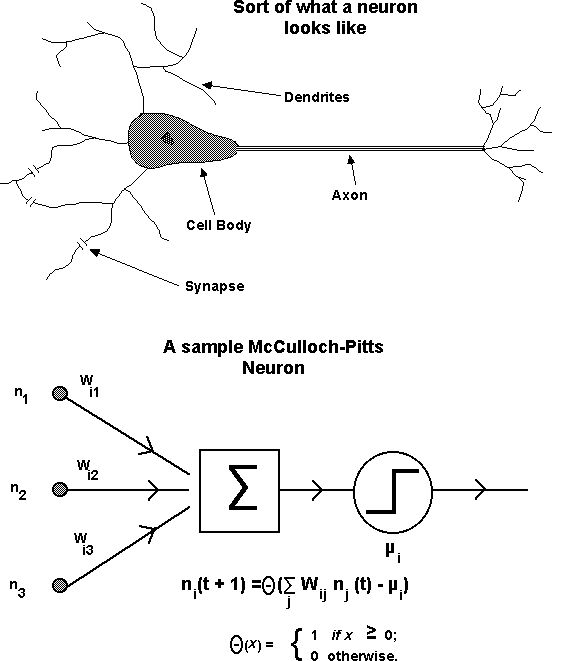
\includegraphics[scale=0.4]{Neuron.JPG}\caption{A biological and mathematical model of a neuron.\cite{key-2}}

\end{figure}



\subsubsection{Feed-Forward Neural Networks}

Feed-forward networks are the most basic form of ANN. A feed-forward
network only contains forward paths%
\footnote{Data only flows in one direction; there are no cycles.%
}. A feed-forward network can be either single-layer (no hidden layers),
or multi-layer (there exists at least one hidden layer). This project
consists of a multi-layer feed-forward network.


\subsubsection{Error-Correction Learning}

Error-correction learning is used with supervised learning systems.
It is the technique of comparing the actual output to the desired
or expected output, and using that error to train ANNs by adjusting
the weights with help of the error values. Error-correction learning
attempts to minimize this error signal with each training iteration.
The most popular learning algorithm (and the one used in this project)
is the backpropagation algorithm (see section~\vref{sub:Error-Backpropagation}).


\subsubsection{Error Backpropagation\label{sub:Error-Backpropagation}}

The main problem with early neural nets was that they could only deal
with linear problems. Researchers knew however that they could overcome
this limitation by adding one or more hidden layers. The problem was
that there was no way to automatically adjust the weights in the hidden
layer in case of errors; there was no learning algorithm. This caused
the decline in interest in neural nets. The revival was due to error
backpropagation%
\footnote{Backpropagation was around since the 1950s but only gained acceptance
in the mid 1980s%
}.

In short, backpropagation networks consist of:
\begin{enumerate}
\item multiple layers of non-linear units
\item computation of an error signal%
\footnote{A backpropagation network uses supervised learning to calculate the
difference between the output and expected output.%
} using the rate of change%
\footnote{That is the derivative.%
} of the non-linear function
\item backpropagation of an error signal
\item estimation of an error signal by the hidden units
\end{enumerate}
Just like a linear unit, the non-linear unit computes its activation
by summing all the weighted activations it receives. However, unlike
the linear unit, it will create a response by putting this sum through
a non-linear transfer function (also known as a sigmoid function or
activation function) which is mentioned in step 2 above. If threshold
is used, then the threshold value is added to the sum before going
through the transfer function. Several transfer functions exist. For
an output range of {[}0, 1{]}, the \emph{logistic function} is used:
$f(x)=logist(x)=\frac{1}{1+e^{-x}}$ This is also the function used
in this project.

The algorithm for backpropagation can be broken down into the following
high-level steps:
\begin{enumerate}
\item Initialize the network with small random weights%
\footnote{Note that if \emph{all} the weights are zero, then the error term
is zero and that means no learning because the correction of the weights
will then be equal to 0.%
}
\item Present an input pattern to the input layer
\item Feed the input pattern forward through the network to calculate its
activation value (i.e. generate a forward flow of activation)
\item Take the difference between desired output and the activation value
to calculate the network's activation error (i.e. compute the error
term)
\item Adjust the weights feeding the output neuron to reduce its activation
error for this input pattern
\item Propagate an error value back to each hidden neuron that is proportional
to their contribution of the network's activation error
\item Adjust the weights feeding each hidden neuron to reduce their contribution
of error for this input pattern
\item Repeat steps 2 to 7 for each input pattern in the input collection
\item Repeat step 8 until desired epochs reached or until the network is
trained to satisfaction
\end{enumerate}

\subsection{Parity Checking}

Parity checking is a simple form of error detection. A parity bit
is an extra bit that is added to a given set of bits. There are two
varients of parity bits: odd parity \& even parity. In odd parity,
if the number of ones in a given set of bits is \emph{even}, the parity
bit is set to 1, which results in the total amount of ones in the
bit data set being \emph{odd}. In even parity, if the number of ones
in a given set of bits is \emph{odd}, the parity bit is set to 1,
which results in the total amount of ones in the bit data set being
\emph{even}.

The standard in computer memory is odd parity, however, this project
focuses on an even parity bit.


\section{Network Parameters}

Parameter values play a big role in the success of an ANN, and there
are many different parameters that must be decided on when designing
a neural network. These parameters include (but not limited to):
\begin{itemize}
\item the number of layers
\item the number of neurons per layer%
\footnote{That is, in the input layer, hidden layer(s) if any, and the output
layer.%
}
\item the number of training iterations
\item the learning rate
\item the momentum
\end{itemize}

\subsection{Number of Hidden Layers}

For most non-linear problems, selecting one hidden layer is sufficient.
It is said that two hidden layers are required for modeling data with
discontinuities and that there is no theoretical reason to use more
than two hidden layers~\cite{key-3}. Adding a hidden layer enlarges
the space of hypotheses that the network can represent.


\subsection{Number of Neurons per Layer}

The number of units in the input layer should be adequate to the number
of variables of which a pattern consists of. This is because each
variable is presented to an input unit.

The number of hidden units represent the number of representations
the network can map for every stimuli's input and output pattern association.
If too few hidden units are used, the network will be unable to model
(complex) data completely, resulting in poor results. If too many
hidden units are used, the training time will become very long and
the network may \emph{overfit} the data. This is when the network
performs really well on trained data, but very poorly on unseen data
(i.e. testing data).

The number of output units depends on the classification that the
problem outputs. For boolean classification, a neural net will usually
have a single output unit, where a result over 0.5 is one classification,
and a result below 0.5 is another. A neural net can also have \emph{k}-way
classification (thus \emph{k} classes). This can be done in two ways:
one is to divide a single output unit into \emph{k} portions; the
other way is to have \emph{k} output units, each representing a different
classification.


\subsection{Number of Iterations \& Epochs}

(This subsection isn't finished yet)


\subsection{Learning Rate \& Momentum}

Learning rate is the scaling factor for which all weight adjustments
are made. Momentum ensures a higher probability that a consequent
weight adjustment will be in the same direction.


\section{Training}


\subsection{Types of Training}

Training configures the neural network to produce a desired set of
outputs given a set of inputs. There exist several learning methods
to train a neural net:
\begin{description}
\item [{Supervised~learning}] the system is provided with matching outputs
for the inputs
\item [{Unsupervised~learning}] the system develops its own representation
of the input stimuli
\item [{Reinforcement~learning}] the system learns by feedback (e.g. {}``good''
or {}``bad'')
\end{description}
The set of patterns to be learned is presented to the input units
(usually in random order) and each pattern is learned in turn. Learning
one pattern is called an \emph{iteration}; learning the full set of
patterns is called an \emph{epoch}.


\subsection{A Numerical Example}

The network in this problem implements a 4-bit system, checking for
even parity (see table~\vref{tab:Sample-of-training}).

%
\begin{table}
\begin{tabular}{|c|c|}
\hline 
input pattern & expected output\tabularnewline
\hline
\hline 
0000 & 0\tabularnewline
\hline 
0001 & 1\tabularnewline
\hline 
... & ...\tabularnewline
\hline 
1111 & 0\tabularnewline
\hline
\end{tabular}\caption{Sample of training data for 4-bit parity checking.\label{tab:Sample-of-training}}

\end{table}
To make the example easy to follow, figures of the network have been
included. A three-layer network, made up of a$_{\text{k}}$= 4 input
units, a$_{\text{j}}$= 4 hidden units, and a$_{\text{i}}$= 1 output
unit (see Fig. \vref{fig:Network-architecture}) will be trained to
associate the stimulus \textbf{x} = {[}0 0 0 1{]} to the response
\textbf{t} = {[}1{]}. To keep the example simple, no threshold is
used. {[}this section isn't finished yet!{]}

%
\begin{figure}
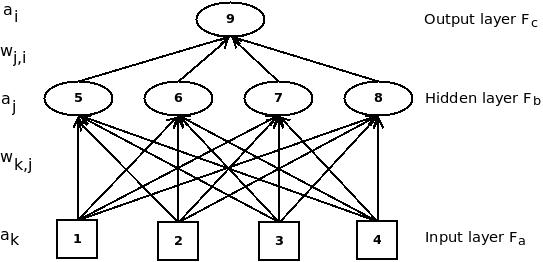
\includegraphics[scale=0.5]{4-4-1-ANN(v2).jpeg}\caption{Network architecture used for this problem (supervisor not visible).\label{fig:Network-architecture}}

\end{figure}



\section{Testing}

{[}section not finished{]}


\section{Stuff from board -- need to incorporate later}
\begin{enumerate}
\item Each unit first computes a weighted sum of its inputs, that is, the
sum of the products of the weights and the inputs $in_{i}=\sum_{j-0}^{n}w_{j,i}*a_{j}$
if threshold is used then $in_{i}=\sum_{j-0}^{n}w_{j,i}*a_{j}+threshold$
\item Then it applies an activation function \emph{g} to this sum to derive
the output $a_{i}=g(in_{i})=g(\sum_{j-0}^{n}w_{j,i}*a_{j})$
\item \emph{g} is the sigmoid function, which in this case is the logistic
function $f(x)=\frac{1}{(1+e^{-x})}$
\end{enumerate}
Then for a 4-4-1 feedforward net:
\begin{enumerate}
\item Given an input vector $x=(x_{1},x_{2},x_{3},x_{4})$, the activations
of the input units are set to $(a_{1},a_{2},a_{3},a_{4})=(x_{1},x_{2},x_{3},x_{4})$.
\item The output unit \emph{a$_{\text{9}}$} (in the output layer \emph{Fc})
will have the activation $a_{9}=g(w_{5,9}a_{5}+w_{6,9}a_{6}+w_{7,9}a_{7}+w_{8,9}a_{8})$
\item Rewrite the function to express the output of each hidden unit as
a function of its inputs (i.e. show the output of the network as a
whole) $a_{9}=g(w_{5,9}g(w_{1,5}a_{1}+w_{2,5}a_{2}+w_{3,5}a_{3}+w_{4,5}a_{4})+w_{6,9}g(w_{1,6}a_{1}+w_{2,6}a_{2}+w_{3,6}a_{3}+w_{4,6}a_{4})$$+w_{7,9}g(w_{1,7}a_{1}+w_{2,7}a_{2}+w_{3,7}a_{3}+w_{4,7}a_{4})+w_{8,9}g(w_{1,8}a_{1}+w_{2,8}a_{2}+w_{3,8}a_{3}+w_{4,8}a_{4}))$
\item Because there is a single output unit, the result will go through
boolean classification. If the value is greater than 0.5, then the
parity bit is 1, otherwise the parity bit is 0.
\end{enumerate}

\section{Conclusion}

{[}section not finished, but basically, parity bit is a bad problem
for NNs because NNs are good for recognizing patterns but a small
change in bit data results in a completely different parity bit{]}
\begin{thebibliography}{DTREG}
\bibitem{key-1}http://upload.wikimedia.org/wikipedia/commons/thumb/e/e4/Artificial\_neural\_network.svg/400px-Artificial\_neural\_network.svg.png

\bibitem{key-2}http://www.bordalierinstitute.com/images/Neuron.JPG

\bibitem[DTREG]{key-3}http://www.dtreg.com/mlfn.htm
\end{thebibliography}

\end{document}
